% !TEX TS-program = xelatex
% !TEX encoding = UTF-8
\documentclass{QHUthesis}
\graphicspath{{figures/}} %设置图片路径
\usepackage{newtxtext}
\usepackage{lipsum}
\usepackage{zhlipsum}
\usepackage[sort&compress]{gbt7714}
\bibliographystyle{gbt7714-numerical}

\begin{document}
	
%%%封面内容
\renewcommand{\title}{The sunset is like a rustling duck, and the autumn water is like a long sky} % 英文标题
\renewcommand{\biaoti}{落霞与孤鹜齐飞秋水共长天一色}  % 中文标题
\renewcommand{\xueyuan}{机械工程学院}
\renewcommand{\zhuanye}{机械电子工程}
\renewcommand{\xingming}{coffeelize}
\renewcommand{\xuehao}{1700417035}
\renewcommand{\grade}{2017级}
\renewcommand{\daoshi}{Coffeelize}
\renewcommand{\dateOfGrant}{2021年5月20日}
\renewcommand{\class}{本科生毕业论文} %毕业论文or毕业设计

%%======生成封面
\titlepage
\thispagestyle{empty} 
%\newblankpage%插入一个新的空白页
%======插入诚信责任书
\statement
\clearpage
%\newblankpage%插入一个新的空白页
\clearpage
%======生成目录
\thispagestyle{empty} 
\tableofcontents
\thispagestyle {empty}

\frontmatter

%======文章主体
\mainmatter %开启章节序号计数,重置页码,页码使用阿拉伯数字;
\songti\zihao{-4} %正文字体为小四号宋体

%%% 中文摘要
\begin{zhAbsract}{关键词1;关键词2}
	\zhlipsum[1]
\end{zhAbsract}
%%% 英文摘要
\begin{enAbsract}{keyword1; keyword2}
	\lipsum[1]
\end{enAbsract}


\chapter{时运不齐,命途多舛}
\section{冯唐易老,李广难封}
\zhlipsum[1-3]
\section{老当益壮,宁移白首之心}
\zhlipsum[1-5]

\begin{figure}[htbp]
	\centering
	\subfigure[subfig:1]{
		\includegraphics[width=0.48\textwidth]{example-image-A}
	}
	\subfigure[subfig:2]{
		\includegraphics[width=0.48\textwidth]{example-image-A}
	}
	\bicaption{两张图片并列}{Two images side by side}
%	\caption{两张图片并列}
	\label{fig:1}
\end{figure}

\section{穷且益坚,不坠青云之志}
\subsection{三尺微命,一介书生}
这是参考论文引用样式\cite{kocher99,cnproceed}

\zhlipsum[1-3]
\chapter{豫章故郡,洪都新府}
\section{千里逢迎}
\zhlipsum[1-3]

\begin{table}
	\centering
	\bicaption{表格供测试使用}{Forms for testing purposes}
	\begin{tabular}{|c|c|c|}
		\hline
		\textbf{姓名} & \textbf{年龄} & \textbf{城市} \\
		\hline
		John & 25 & London \\
		\hline
		Alice & 30 & New York \\
		\hline
		Bob & 35 & Paris \\
		\hline
		\multicolumn{3}{|c|}{表格供测试使用} \\ 
		\hline
	\end{tabular}
	\label{tab:1}
\end{table}

如表\ref{tab:1}所示,\zhlipsum[1]


\section{高朋满座}

\begin{figure}[htbp]
	\centering
	\subfigure[subfig:1]{
		\includegraphics[width=0.3\textwidth]{example-image-A}
	}
	\subfigure[subfig:2]{
		\includegraphics[width=0.3\textwidth]{example-image-A}
	}
	\subfigure[subfig:3]{
		\includegraphics[width=0.3\textwidth]{example-image-A}
	}
	\caption{两张图片并列}
	\label{fig:subfigure_example1}
\end{figure}

\zhlipsum[1-5]
\section{腾蛟起凤,孟学士之词宗}
\chapter{格式调整}
\zhlipsum[1]

\begin{table}
	\centering
	\begin{tabular}{|c|l|}
		\hline
		\textbf{命令} & \textbf{效果} \\
		\hline
		\verb|\tiny| & {\tiny 这是 \texttt{tiny} 字号} \\
		\hline
		\verb|\scriptsize| & {\scriptsize 这是 \texttt{scriptsize} 字号} \\
		\hline
		\verb|\footnotesize| & {\footnotesize 这是 \texttt{footnotesize} 字号} \\
		\hline
		\verb|\small| & {\small 这是 \texttt{small} 字号} \\
		\hline
		\verb|\normalsize| & {\normalsize 这是 \texttt{normalsize} 字号} \\
		\hline
		\verb|\large| & {\large 这是 \texttt{large} 字号} \\
		\hline
		\verb|\Large| & {\Large 这是 \texttt{Large} 字号} \\
		\hline
		\verb|\LARGE| & {\LARGE 这是 \texttt{LARGE} 字号} \\
		\hline
		\verb|\huge| & {\huge 这是 \texttt{huge} 字号} \\
		\hline
		\verb|\Huge| & {\Huge 这是 \texttt{Huge} 字号} \\
		\hline
	\end{tabular}
\end{table}

文献引用\cite{cnproceed},可以使用\textbackslash cite\{cnproceed\}的形式引用

\zhlipsum[1]

\section{潦水尽而寒潭清}
\zhlipsum[1-5]
\section{烟光凝而暮山紫}


\chapter{特殊符号}

\section{带圈数字}

\begin{figure}[htbp]
	\centering
		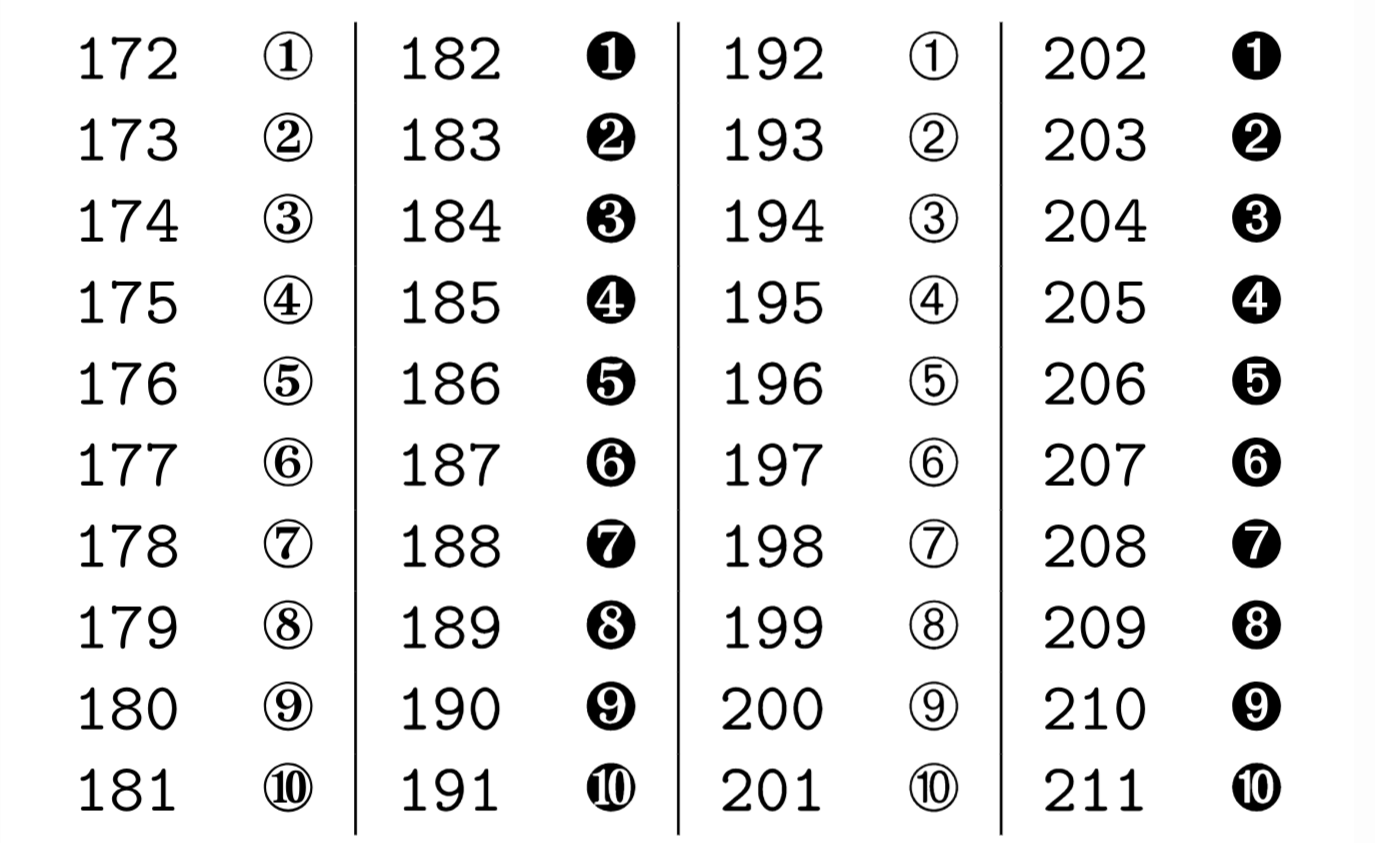
\includegraphics[width=\textwidth]{带圈数字符号}
	\caption{带圈数字符号}
	\label{fig:2}
\end{figure}

比如\ding{172}、\ding{181}符号,在 \LaTeX 中,使用 \textbackslash ding\{172\}  命令即可生成。

\zhlipsum[1-3]
\section{落霞与孤鹜齐飞,秋水共长天一色}
\zhlipsum[1-5]

\chapter{章节标题}
\section{一级节标题}
\subsection{二级节标题}
\subsection{二级节标题}
\subsubsection{三级节标题}
\subsubsection{三级节标题}
\section{一级节标题}
\subsection{二级节标题}
\subsection{二级节标题}
\subsubsection{三级节标题}
\subsubsection{三级节标题}
\section{一级节标题}
\subsection{二级节标题}
\subsection{二级节标题}
\subsubsection{三级节标题}
\subsubsection{三级节标题}
\section{一级节标题}
\subsection{二级节标题}
\subsection{二级节标题}
\subsubsection{三级节标题}
\subsubsection{三级节标题}
\paragraph{段落标题}
\paragraph{段落标题}

\chapter{章节标题}
\zhlipsum[1]
\section{一级节标题}
\zhlipsum[1]
\subsection{二级节标题}
\zhlipsum[1]
\subsubsection{三级节标题}
\zhlipsum[1]
\paragraph{段落标题}
\zhlipsum[1]
\subparagraph{子段落标题}
\zhlipsum[1]



%=======论文后部=======
\backmatter
%=======参考文献
\bibliography{reference} 
\addcontentsline{toc}{chapter}{参考文献}


%%% 致谢
\Thanks
\zhlipsum[1]
%%%附录
%\makeappedixfigtabnum %重新计算附图和表的标题号和计数号
\Appendix
\zhlipsum[1]

\end{document}